% CEG5101 CA2 report -- compile with:  latexmk -pdf report.tex   (run inside report/)
\documentclass[11pt,a4paper]{article}

\usepackage[T1]{fontenc}
\usepackage[utf8]{inputenc}
\usepackage{lmodern}
\usepackage[margin=2.2cm]{geometry}
\usepackage{microtype}
\usepackage{amsmath,amssymb}
\usepackage{graphicx}
\usepackage{booktabs}
\usepackage{tabularx}
\usepackage{array}
\usepackage{float}
\usepackage{caption}
\usepackage{enumitem}
\usepackage{xcolor}
\usepackage{listings}
\usepackage{tikz}
\usetikzlibrary{arrows.meta,positioning,calc}
\usepackage[hidelinks]{hyperref}

\captionsetup{font=small,labelfont=bf}
\setlist{itemsep=2pt,topsep=4pt}
\setlength{\parskip}{4pt}
\setlength{\parindent}{0pt}
\setlength{\emergencystretch}{3em}

\definecolor{accent}{HTML}{2A78D6}
\definecolor{edge}{HTML}{898781}
\definecolor{codebg}{HTML}{F5F5F3}

\lstset{basicstyle=\ttfamily\small,backgroundcolor=\color{codebg},frame=none,
        breaklines=true,columns=fullflexible,keepspaces=true,xleftmargin=4pt}

\newcommand{\ra}{\ensuremath{\rightarrow}}
\newcommand{\code}[1]{\texttt{#1}}
\newcommand{\Czero}{\ensuremath{C^{0}}}
\newcommand{\figref}[1]{Figure~\ref{#1}}
\newcommand{\tabref}[1]{Table~\ref{#1}}

\title{\textbf{CEG5101 CA2 Laboratory Assignment}\\[4pt]
       \large Anomaly-aware Routing and Blocking Controller}
\author{Group 5\\[2pt] Yang Kaiming (A0326309E)\qquad Chen Danze (A0328226E)}
\date{November 2026}

\begin{document}
\maketitle

\begin{abstract}
\noindent
An integrated Ryu controller was built that monitors per-source traffic, detects ICMP floods with an
exponential-moving-average baseline, blocks the offending source IP, and reroutes legitimate traffic using a
dynamic link cost that combines load and anomaly status. In three repeated runs on the provided 6-switch mesh,
every flood was detected and blocked within 1.5--3.8\,s, after which no attack packet reached the victim. The
legitimate h1\ra h6 flow stayed connected throughout; it was rerouted only in the case where the attack shared
its path (case~b), and it returned to its original path 13.6--14.9\,s after the flood ended. A further run on
the official Mininet VM, with the kernel datapath and real link delays, blocked the same hosts, marked the same
links and again rerouted h1\ra h6 only in case~b.
\end{abstract}

% =====================================================================
\section{Introduction}

The integrated controller detected and blocked every ICMP flood within 1.5--3.8\,s and kept the legitimate
h1\ra h6 flow connected in all three cases. In case~b it moved h1\ra h6 to a backup path and moved it back after
the attack. The attacker's packets stopped reaching the victim within one monitoring interval of detection.

The controller merges the two reference applications, \code{resilient\_controller.py} (topology discovery,
Dijkstra routing) and \code{anomaly\_detection.py} (flow statistics, EMA baseline, IP blocking). It adds three
things neither has:
\begin{itemize}
  \item per-link load measurement from port statistics;
  \item a dynamic link cost that combines load and anomaly status (Eq.~\ref{eq:cost});
  \item proactive, path-wide rerouting of legitimate flows, with recovery once the anomaly ends.
\end{itemize}

\paragraph{Environment.} Runs R1--R3 used Mininet 2.3.0, Open vSwitch 3.3.9, Ryu 4.34 on Python 3.9, OpenFlow
1.3, iperf 2.1.9 and hping3 3.0.0-alpha-2 on Ubuntu 24.04 in a container. The container had no OVS kernel module,
so OVS used its userspace datapath. Its kernel also lacked \code{sch\_netem}: the 40\,Mbps bandwidth limits
applied, but link delays could not be emulated. Routing costs are held in the controller, so path selection is
unaffected; only absolute RTT values are smaller than on a standard Mininet VM.

The experiment and the Task~1 MiniEdit build were then repeated on the official Mininet 2.3.0 VM image
(Ubuntu 20.04, kernel 5.4, OVS 2.13 with its kernel datapath, \code{sch\_netem}, Python 3.8), with Ryu 4.34
installed by the same \code{support/environment/setup\_ubuntu.sh}. The VM ran inside the container under QEMU 8.2 with pure
software emulation (no KVM), 4 virtual CPUs and 4\,GB of RAM (\code{support/environment/qemu\_mininet\_vm.sh}). This checks
the setup the assignment expects: the kernel datapath, real link delays and RTTs, and MiniEdit on the standard
VM. It does not check performance. The emulated CPU limited how fast the attacker could send, so the flood was
weaker than in R1--R3 and the loss figures of the two environments are not comparable (Section~\ref{sec:vm}).

% =====================================================================
\section{Topology (Task 1)}

The topology from \code{ceg\_mesh\_topo.py} was built through MiniEdit's GUI on the Mininet 2.3.0 VM
(Section~1) and run there with a remote controller (127.0.0.1:6633, OpenFlow~1.3). \code{pingall} reached all 30
host pairs with 0\% loss, and \code{h1 ping -c 4 h6} averaged 101.3\,ms over the emulated link delays
(Figures~\ref{fig:miniedit-canvas} and~\ref{fig:miniedit-run}). Six switches each serve one host (h$_i$ on
s$_i$, 10.0.0.$i$/24) over 40\,Mbps, 15\,ms links. Eleven 40\,Mbps switch-to-switch links form a redundant mesh,
and each link's delay in ms is its static routing cost \Czero{} (\tabref{tab:c0}).

\begin{figure}[H]
  \centering
  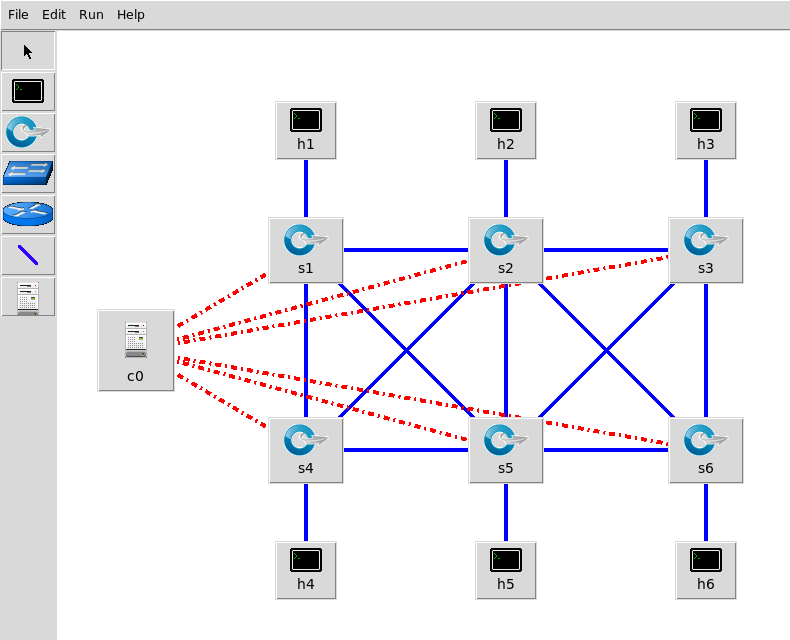
\includegraphics[width=0.48\textwidth]{figures/task1_miniedit_canvas.png}
  \caption{MiniEdit canvas in the Mininet 2.3.0 VM after the GUI build (saved as \code{my\_topology.mn}): six
  switches, six hosts, eleven mesh links and the remote controller c0 with its six control links (red).}
  \label{fig:miniedit-canvas}
\end{figure}

\begin{figure}[H]
  \centering
  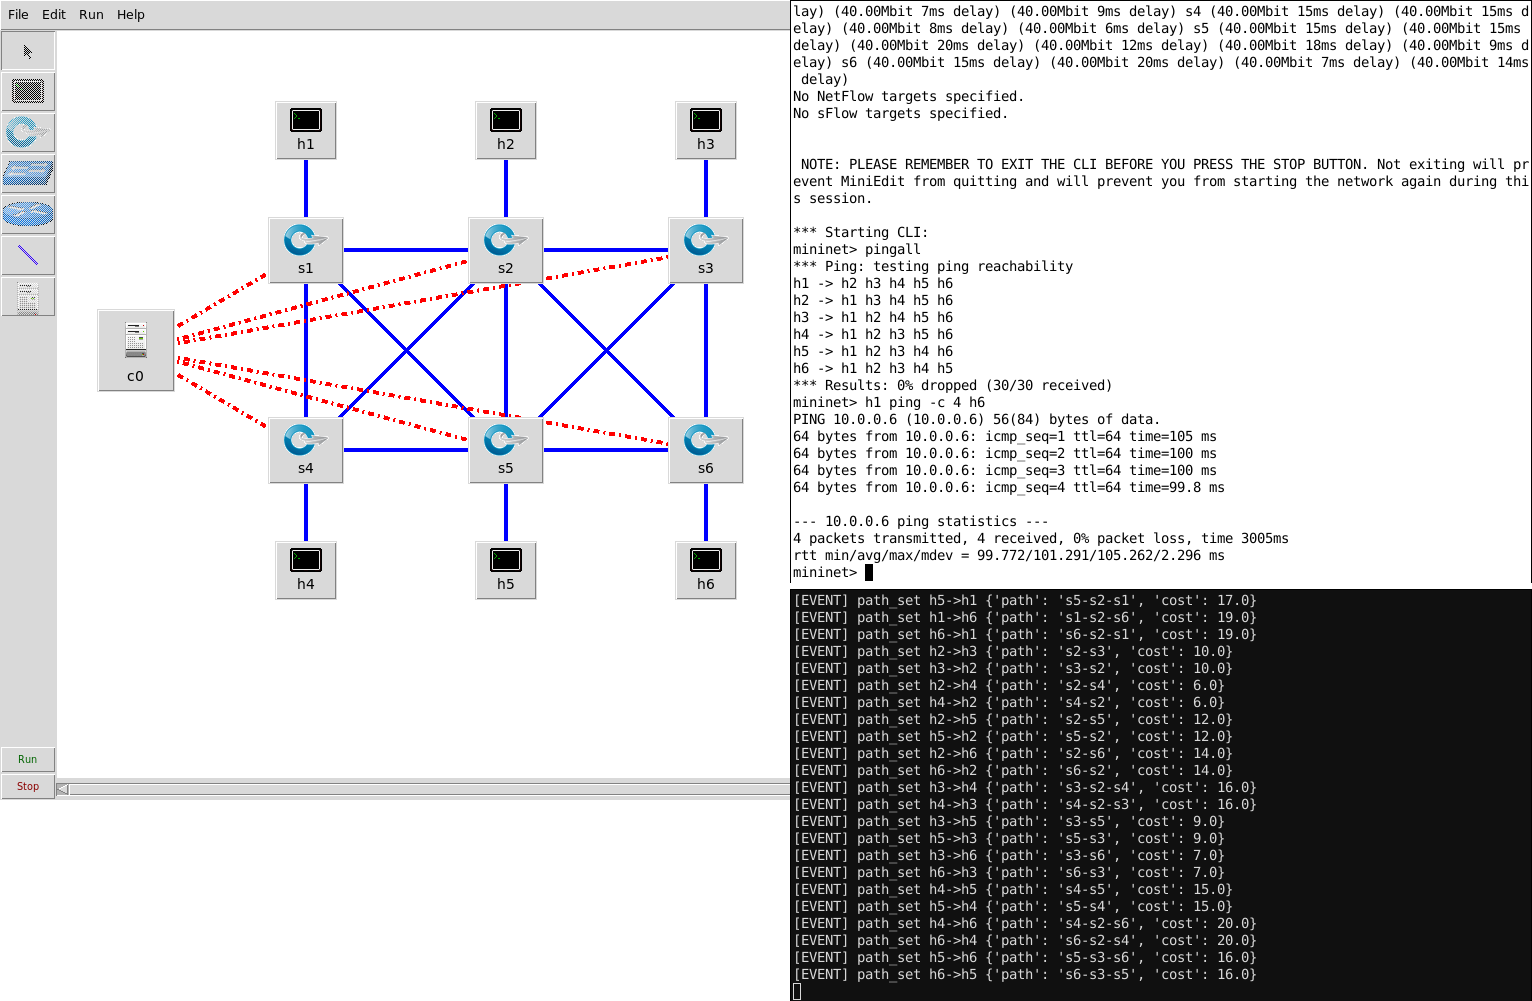
\includegraphics[width=\textwidth]{figures/task1_miniedit_running.png}
  \caption{The MiniEdit network running in the VM (toolbar disabled). Top right: MiniEdit's CLI, with each
  link's emulated delay, \code{pingall} at 0\% dropped (30/30) and \code{h1 ping -c 4 h6} at
  99.8/101.3/105.3\,ms (min/avg/max). Bottom right: the controller computes h1\ra h6\,=\,s1-s2-s6 (cost 19).}
  \label{fig:miniedit-run}
\end{figure}

\begin{table}[H]
  \centering
  \caption{Static link costs \Czero{} (= link delay in ms). All links are 40\,Mbps.}
  \label{tab:c0}
  \begin{tabular}{lr@{\qquad}lr}
    \toprule
    Link & \Czero{} (ms) & Link & \Czero{} (ms) \\
    \midrule
    s1--s2 & 5  & s2--s5 & 12 \\
    s2--s4 & 6  & s2--s6 & 14 \\
    s3--s6 & 7  & s4--s5 & 15 \\
    s1--s4 & 8  & s1--s5 & 18 \\
    s3--s5 & 9  & s5--s6 & 20 \\
    s2--s3 & 10 &        &    \\
    \bottomrule
  \end{tabular}
\end{table}

With these costs h1\ra h6 takes s1-s2-s6 (cost 19); the next best path is s1-s2-s3-s6 (cost 22). The attack
flows of the three cases take s2-s3 (h2\ra h3), s2-s6 (h2\ra h6) and s5-s3-s6 (h5\ra h6, cost 16, cheaper than
the direct s5-s6 at 20). So only case~b overlaps h1\ra h6, and only case~b should make it reroute.

The topology was entered through the GUI of the MiniEdit shipped with Mininet 2.3.0. Switches, hosts and c0
were placed with the toolbar tools, and the 17 data links and 6 control links were drawn on the canvas. Each
link's bandwidth (40\,Mbps) and delay were typed into its Link Details dialog and each host's address into Host
Properties, and c0 was set to Remote Controller at MiniEdit's default 127.0.0.1:6633. Under
\emph{Edit\,\ra\,Preferences} only OpenFlow~1.3 and Start CLI were enabled. \emph{File\,\ra\,Save} wrote
\code{code/miniedit/my\_topology.mn}, and a script check found that its links, bandwidths, delays and addresses equal
those of \code{ceg\_mesh\_topo.py}. \emph{File\,\ra\,Export Level~2 Script} wrote
\code{support/miniedit/my\_topology\_export.py}.

Screenshots of each step and a 7-minute screen recording of the build are in \code{results/miniedit-vm/}.
In the run shown, OVS used its kernel datapath and every link had
its delay: MiniEdit's console lists each link as, for example, \code{(40.00Mbit 15ms delay)}, and the ping times
of 99.8--105.3\,ms fit the 98\,ms that the delays of s1-s2-s6 add up to.

Two MiniEdit problems are worth knowing. Under Python~3, \emph{Save} and \emph{Export} fail and leave an empty
file, because \code{miniedit.py} opens the file in binary mode; changing the mode \code{wb} to \code{w} in those
two \code{open()} calls fixes it. The exported script also drops the OpenFlow~1.3-only setting. It still works
with Ryu because OVS~2.13 enables OpenFlow~1.0--1.5 by default, but a \code{protocols} argument can be added to
its \code{addSwitch} calls.

% =====================================================================
\section{Controller design}

The controller turns flow and port statistics into one routing decision every 2\,s: who is attacking, which links
they load, what each link costs now, and whether any legitimate flow should move (\figref{fig:loop}).

\begin{figure}[H]
\centering
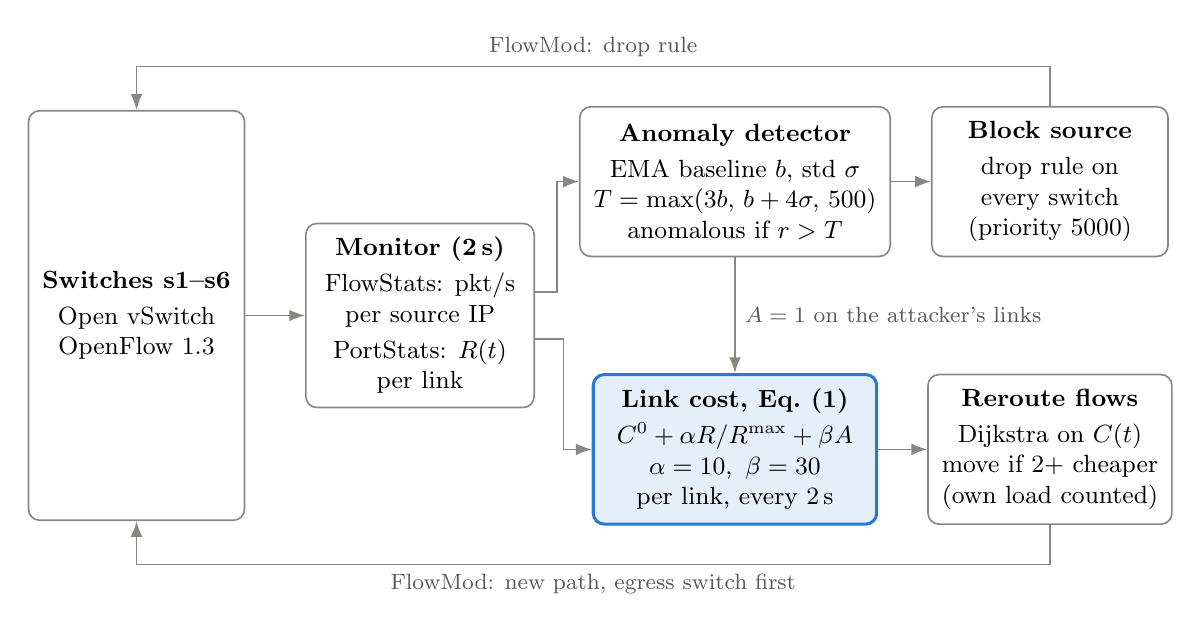
\begin{tikzpicture}[
  font=\small,
  box/.style={draw=edge,rounded corners=4pt,line width=0.6pt,align=center,inner sep=5pt},
  main/.style={box,draw=accent,line width=1.1pt,fill=accent!12},
  arr/.style={-{Latex[length=2mm]},draw=edge,line width=0.6pt},
  lbl/.style={font=\footnotesize,text=black!65}]
  \node[box,minimum width=2.6cm,minimum height=5.2cm] (sw) at (0,0)
       {\textbf{Switches s1--s6}\\[2pt]Open vSwitch\\OpenFlow 1.3};
  \node[box,minimum width=2.9cm] (mon) at (3.6,0)
       {\textbf{Monitor (2\,s)}\\[2pt]FlowStats: pkt/s\\per source IP\\[2pt]PortStats: $R(t)$\\per link};
  \node[box,minimum width=3.6cm,minimum height=1.9cm] (det) at (7.6,1.7)
       {\textbf{Anomaly detector}\\[2pt]EMA baseline $b$, std $\sigma$\\$T=\max(3b,\,b+4\sigma,\,500)$\\anomalous if $r>T$};
  \node[box,minimum width=3.0cm,minimum height=1.9cm] (blk) at (11.6,1.7)
       {\textbf{Block source}\\[2pt]drop rule on\\every switch\\(priority 5000)};
  \node[main,minimum width=3.6cm,minimum height=1.9cm] (cost) at (7.6,-1.7)
       {\textbf{Link cost, Eq.~(1)}\\[2pt]$C^0+\alpha R/R^{\max}+\beta A$\\$\alpha=10,\ \beta=30$\\per link, every 2\,s};
  \node[box,minimum width=3.0cm,minimum height=1.9cm] (rr) at (11.6,-1.7)
       {\textbf{Reroute flows}\\[2pt]Dijkstra on $C(t)$\\move if 2+ cheaper\\(own load counted)};
  \draw[arr] (sw.east) -- (mon.west);
  \draw[arr] (mon.east) ++(0,0.3) -| ($(mon.east)!0.5!(det.west|-mon.east)+(0,0.3)$) |- (det.west);
  \draw[arr] (mon.east) ++(0,-0.3) -| ($(mon.east)!0.5!(cost.west|-mon.east)+(0,-0.3)$) |- (cost.west);
  \draw[arr] (det) -- node[right,lbl] {$A=1$ on the attacker's links} (cost);
  \draw[arr] (det) -- (blk);
  \draw[arr] (cost) -- (rr);
  \draw[arr] (blk.north) -- ++(0,0.5) -| node[pos=0.25,above,lbl] {FlowMod: drop rule} (sw.north);
  \draw[arr] (rr.south) -- ++(0,-0.5) -| node[pos=0.25,below,lbl] {FlowMod: new path, egress switch first} (sw.south);
\end{tikzpicture}
\caption{One 2\,s control loop turns switch statistics into blocking and rerouting. The detector and the cost
model share one signal: when a source is blocked, the links its traffic used get $A=1$, which is what moves
legitimate flows away.}
\label{fig:loop}
\end{figure}

\subsection{Forwarding and topology}
\begin{itemize}
  \item \textbf{Topology.} Ryu's LLDP discovery (\code{-{}-observe-links}) builds a switch graph
        that maps each switch and neighbour to the local output port. Ports not in any link are host ports.
  \item \textbf{ARP.} The controller answers ARP requests itself when it knows the target, and otherwise
        delivers the frame only to host-facing ports. Broadcasts never cross switch-to-switch links, so the
        meshed topology cannot loop without a spanning tree. Packet-ins are ignored until all 11 links are
        discovered.
  \item \textbf{Routing.} The first IPv4 packet of a host pair triggers Dijkstra on the current dynamic costs.
        Rules are installed on every switch of the path at once, egress first, so the ingress switch never
        forwards into a switch without a rule. Rules match \code{ipv4\_src}, \code{ipv4\_dst},
        \code{ip\_proto} and, for ICMP, \code{icmpv4\_type}.
\end{itemize}

\subsection{Monitoring and anomaly detection (Task 2)}

Every 2\,s the controller requests flow and port statistics from all switches. A source's packet rate is counted
only at the switch it is attached to, so each packet is counted once. ICMP echo replies are excluded: during a
ping flood the victim answers at the flood rate, and counting that would block the victim instead of the
attacker.

Each source keeps an exponential moving average baseline $b$ ($\alpha=0.3$, as in the reference code) and an
exponentially weighted variance $\sigma^2$. A sample $r$ is anomalous when it exceeds the threshold
\begin{equation}
  T = \max\left(3\,b,\; b + 4\sigma,\; 500\ \text{pkt/s}\right).
  \label{eq:threshold}
\end{equation}
The sample is compared with the threshold before it updates the baseline, and anomalous samples are never
learned. The reference code updates first, which raises the effective threshold to about $21\times$ the old
baseline and lets an attack poison its own baseline. The $\sigma$ term adapts the threshold to how bursty a
source normally is, which addresses the fixed-threshold limitation of the reference detector. The 500\,pkt/s
floor ignores small bursts from near-idle sources. A source must have 5 samples (10\,s) before it can be
flagged; on a network with link delays the experiment runner raises this to 12 (Section~\ref{sec:vm}).

On detection the controller installs a priority-5000 drop rule for that \code{ipv4\_src} on every switch, as
the reference code does.

\subsection{Dynamic link cost (Task 3)}

The cost of link $(i,j)$ follows Eq.~(1) of the assignment:
\begin{equation}
  C_{ij}(t) = C^{0}_{ij} + \alpha\,\frac{R_{ij}(t)}{R^{\max}_{ij}} + \beta\,A_{ij}(t).
  \label{eq:cost}
\end{equation}
\begin{itemize}
  \item \Czero{} is the link's delay in ms from \code{ceg\_mesh\_topo.py} (the reference controller's static cost
        table described an older 4-switch topology and was rewritten).
  \item $R(t)$ is the larger of the two directions' transmit rates from port statistics, smoothed with an EMA
        (weight 0.6); $R^{\max}=40$\,Mbps, the TCLink bandwidth. $R/R^{\max}$ is capped at 1.
  \item $A(t)=1$ on every link of the paths the blocked source was using in the interval that triggered
        detection.
  \item $\alpha=10$ and $\beta=30$. The backup path for h1\ra h6 costs 3 more than the primary, so $\beta$ must
        exceed 3 plus the rerouting margin of 2 to move traffic off an attacked link.
\end{itemize}

Blocking at the ingress removes the attack load within one interval, so the load term alone cannot keep traffic
away from the attacked link. $A(t)$ therefore stays at 1 while the blocked source keeps hitting its drop rule at
more than half the detection threshold, and for 10\,s after that. The rate condition matters: the attacker's
normal 1\,pkt/s ping also hits the drop rule and would otherwise keep the link marked forever. After 10\,s below
that rate the source is unblocked, so later attacks from the same host are detected again.

\subsection{Rerouting and recovery (Task 4)}

After every update the controller checks each active flow. It compares the flow's current path cost with the
best alternative, where the flow's own rate is added to links it does not yet use. Without that correction a
flow's own load makes its current path look worse, and it oscillates between paths. The flow moves only if the
alternative is cheaper by more than a margin of 2.

A move installs the new path egress first, then deletes the flow's rules on switches that are no longer on the
path. When $A(t)$ returns to 0 the same comparison moves the flow back to the original path. Link failures
reported by LLDP make the current path's cost infinite, so failed links are handled by the same rule.

% =====================================================================
\section{Experiment methodology}

Each run is one continuous 4.5-minute timeline, so the three cases share one time axis: 40\,s of normal traffic,
then for each case a 25\,s flood followed by 45\,s of recovery. \nolinkurl{code/experiments/run_experiment.py} builds the
topology, starts the controller and drives all traffic; the full a, b, c timeline was repeated three times
(runs R1--R3), and once more on the Mininet VM with link delays (Section~\ref{sec:vm}).

\noindent\textbf{Traffic.}\par
\begin{itemize}
  \item Legitimate flow: \code{iperf -u -b 10M} from h1 to h6 for the whole run, plus \code{ping -i 0.5}
        h1\ra h6 for RTT. It starts before the baseline period, so h1's baseline is learned from it.
  \item Normal traffic for baselines: 1\,pkt/s pings h2\ra h4, h3\ra h5, h4\ra h1, h5\ra h2 and h6\ra h3.
  \item Attack: \code{hping3 -{}-icmp -{}-flood -d 1000 <victim>}, about 4{,}800\,pkt/s ($\approx$\,39\,Mbps),
        limited by the attacker's 40\,Mbps access link.
\end{itemize}

\noindent\textbf{Metrics.}\par
\begin{table}[H]
  \centering
  \small
  \begin{tabularx}{\textwidth}{>{\raggedright\arraybackslash}X >{\raggedright\arraybackslash}X}
    \toprule
    Metric & Source \\
    \midrule
    Throughput (Mbps), packet loss (\%) of h1\ra h6 & iperf UDP server report on h6, 1\,s intervals \\
    Path of each flow, link rate, $A(t)$, $C(t)$, $C(t)/C^0$ & controller logs every 2\,s
      (\code{paths.csv}, \code{links.csv}) \\
    Detection time, blocked source, anomalous links & controller event log (\code{events.csv}) \\
    Attack packets reaching the victim & \code{tcpdump} on the victim, ICMP from the attacker only \\
    Flow tables & \code{ovs-ofctl dump-flows} before, during and after each flood \\
    \bottomrule
  \end{tabularx}
\end{table}

``Before'' is the 15\,s before a flood, ``during'' is the 25\,s flood, ``after'' is the last 15\,s of recovery.
Detection delay is the time from the start of the flood to the block event.

\noindent\textbf{Parameters.}\par
\begin{table}[H]
  \centering
  \small
  \begin{tabular}{ll}
    \toprule
    Parameter & Value \\
    \midrule
    Polling interval & 2\,s \\
    EMA $\alpha$ (baseline) & 0.3 \\
    Threshold & $\max(3b,\ b+4\sigma,\ 500\ \text{pkt/s})$ \\
    Warm-up & 5 samples (12 with link delays) \\
    Cost weights $\alpha$, $\beta$ & 10, 30 \\
    $R^{\max}$ & 40\,Mbps \\
    Rerouting margin & 2 \\
    Anomaly hold / unblock after quiet & 10\,s / 10\,s \\
    \bottomrule
  \end{tabular}
\end{table}

% =====================================================================
\section{Results (Task 4)}

All nine floods (3 cases $\times$ 3 runs) were detected, the attacker was blocked, and h1\ra h6 stayed
connected. Only case~b changed the h1\ra h6 path, which is what the topology predicts. Values in
\tabref{tab:results} are given as R1\,/\,R2\,/\,R3.

\begin{table}[!htb]
  \centering
  \small
  \caption{Per-case results of the three repeated runs (R1\,/\,R2\,/\,R3).}
  \label{tab:results}
  \footnotesize
  \setlength{\tabcolsep}{4pt}
  \begin{tabularx}{\textwidth}{l l l >{\raggedright\arraybackslash}X l l l}
    \toprule
    Case & Detection (s) & Anomalous links & h1\ra h6 path during flood & Mean loss (\%) &
      Worst 1\,s loss (\%) & Lowest 1\,s Mbps \\
    \midrule
    a: h2\ra h3 & 3.4 / 2.2 / 3.5 & s2-s3 & s1-s2-s6 (unchanged) & 0 / 0 / 0 & 0 / 0 / 0 & 10.5 / 10.5 / 10.5 \\
    b: h2\ra h6 & 3.8 / 2.6 / 1.5 & s2-s6 & \textbf{s1-s2-s3-s6} & 5.67 / 4.20 / 1.87 & 48.4 / 56.6 / 34.4 &
      5.41 / 4.55 / 6.74 \\
    c: h5\ra h6 & 1.7 / 3.0 / 1.8 & s3-s5, s3-s6 & s1-s2-s6 (unchanged) & 0.12 / 0.45 / 0.31 &
      2.5 / 4.1 / 6.1 & 10.0 / 9.88 / 9.65 \\
    \bottomrule
  \end{tabularx}
\end{table}

Before every flood and in the last 15\,s of every recovery, h1\ra h6 ran at 10.5\,Mbps with 0\% loss on
s1-s2-s6.

\subsection{Blocking (Task 2 check)}

No attack packet reached the victim later than 1\,s after the block in any of the nine floods (tcpdump on the
victim, \figref{fig:blocking}). Before the block, 3{,}608--14{,}251 flood packets got through, which is the
flood rate multiplied by the detection delay. The attacker kept sending about 4{,}800\,pkt/s for the whole 25\,s,
and the drop rule on its access switch counted them (for example \code{n\_packets=31253} on s2 six seconds after
the block in case~b, R1).

\begin{figure}[H]
  \centering
  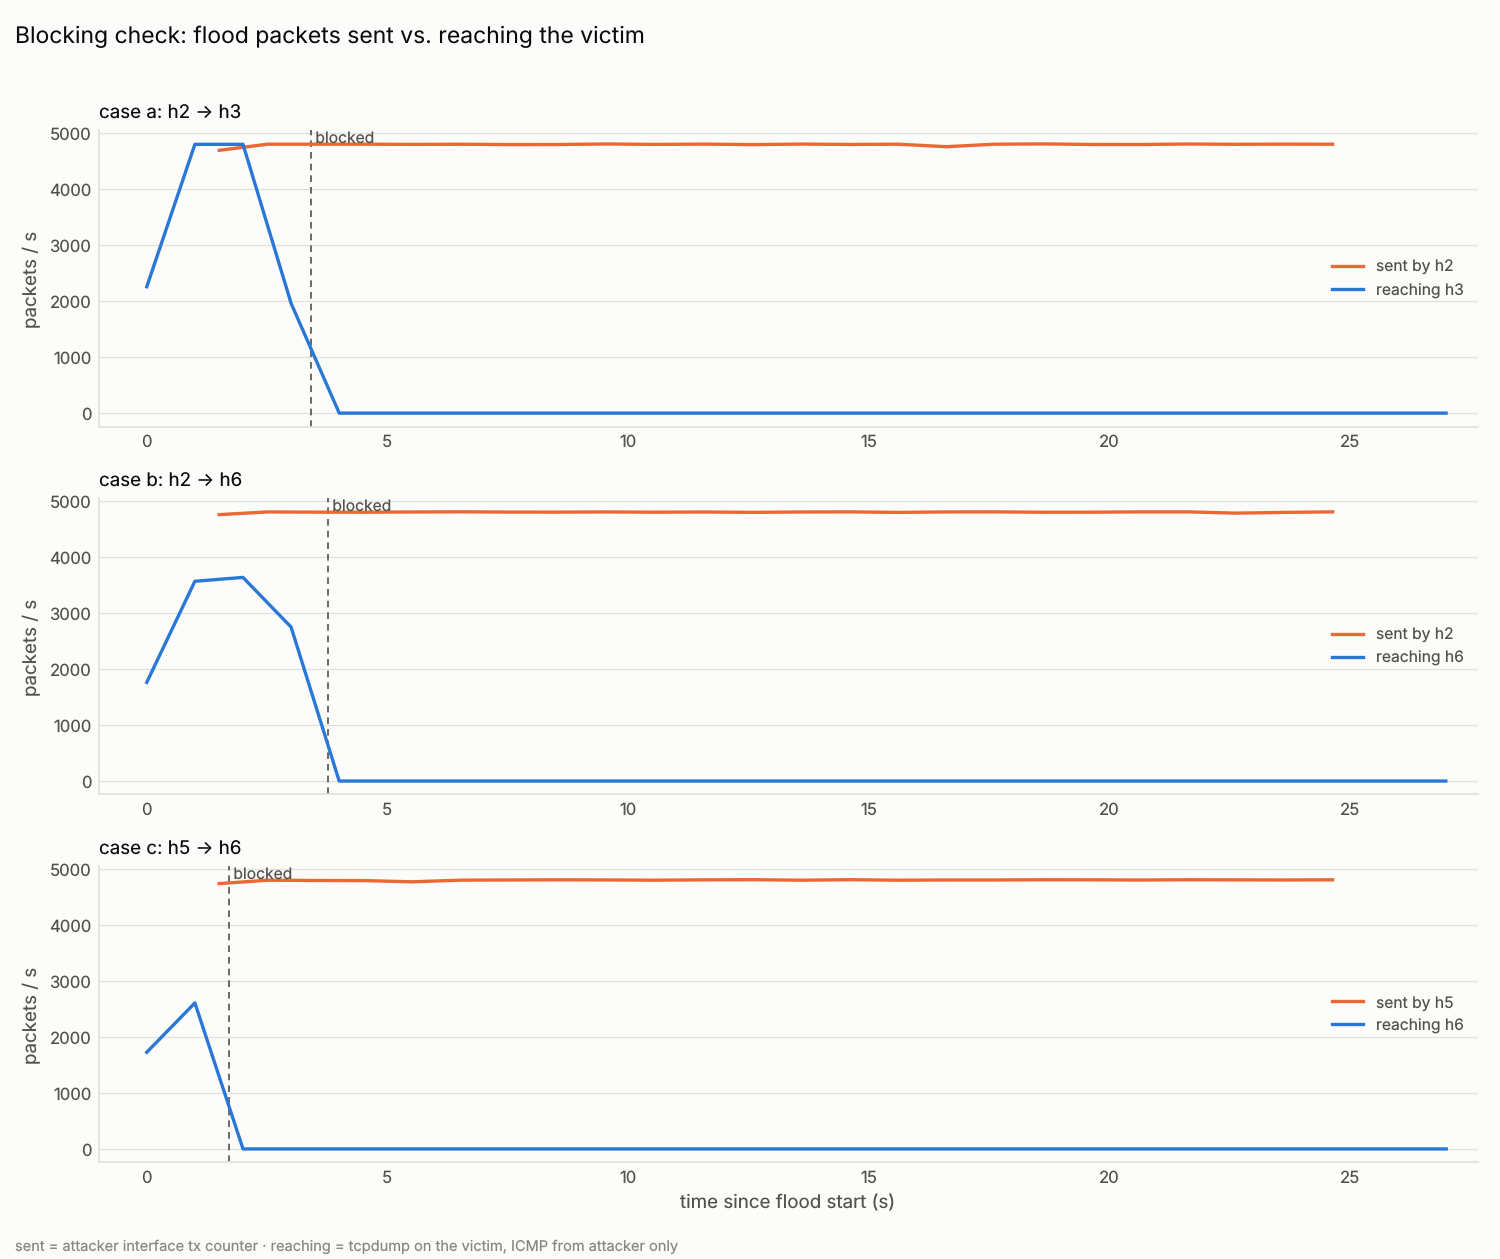
\includegraphics[width=0.92\textwidth]{figures/fig5_blocking.png}
  \caption{R1 blocking check: flood packets sent by the attacker vs.\ packets reaching the victim, per case.}
  \label{fig:blocking}
\end{figure}

The same check was run step by step in a Mininet CLI session (commands from a script, controller events on the
left of \figref{fig:cli}). After 15\,s of 1\,pkt/s ping from h2, \code{hping3 -{}-icmp -{}-flood} was started towards
h3. The drop rule on s2 counted 18{,}951 and then 28{,}521 packets two seconds apart, and \code{tcpdump} on h3
captured 0 attack packets in 3\,s. The controller also moved the legitimate h1\ra h3 flow off the marked link
s2-s3 onto s1-s2-s5-s3.

\begin{figure}[H]
  \centering
  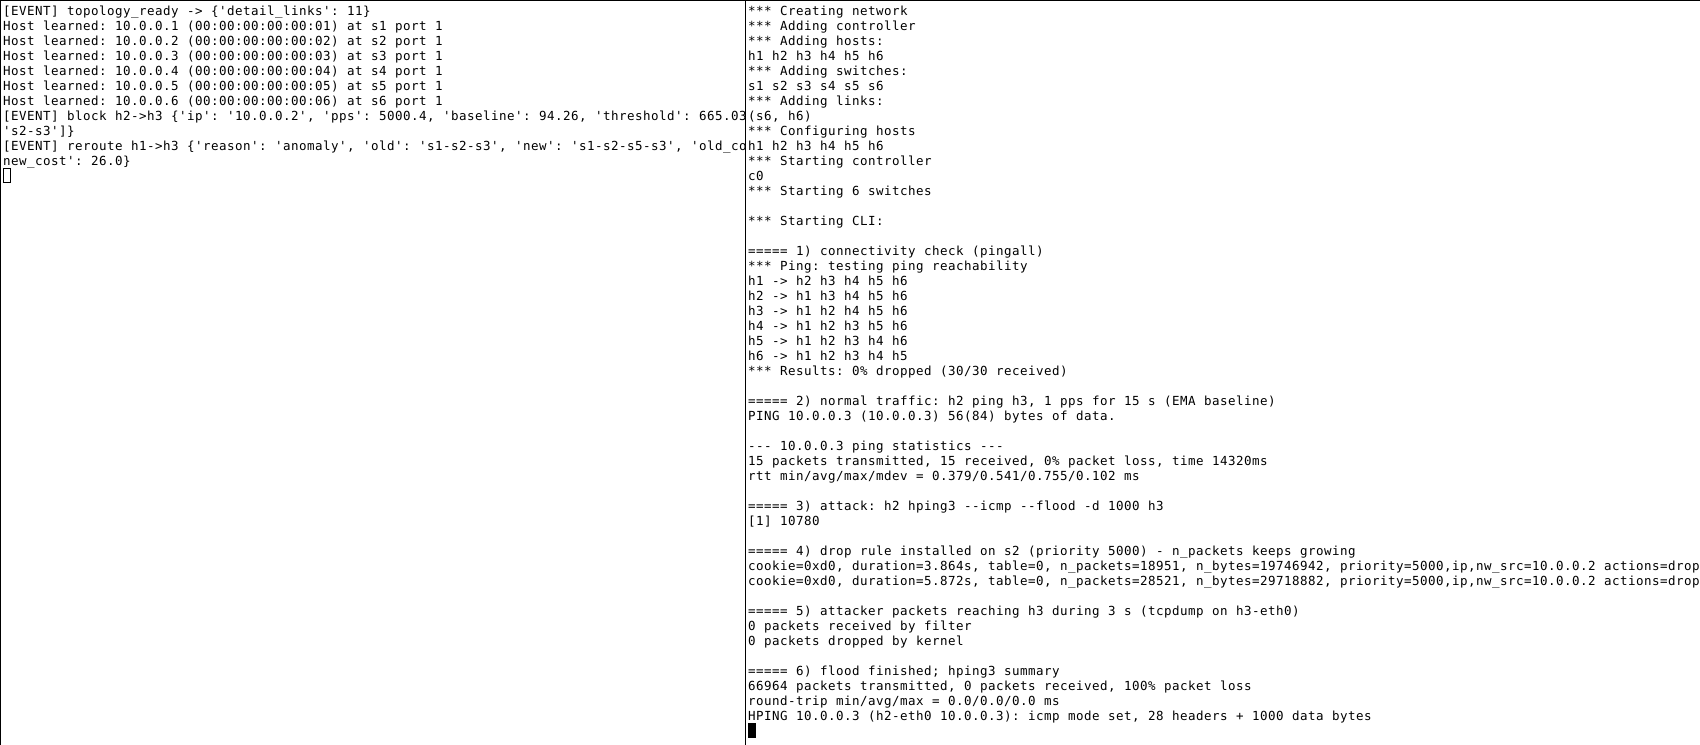
\includegraphics[width=\textwidth]{figures/task2_cli_demo.png}
  \caption{Mininet CLI demonstration of detection and blocking: controller events (left) and CLI output
  (right).}
  \label{fig:cli}
\end{figure}

Detection takes one or two 2\,s polling intervals. If the flood starts late in an interval, the first sample
covers only part of the flood and may stay under the 500\,pkt/s floor, which adds one interval. In R1 case~b the
first sample was 491\,pkt/s, just under the floor, so it was learned: h2's baseline rose from 1 to 148\,pkt/s and
its threshold to 1{,}046\,pkt/s. The next sample, 4{,}994\,pkt/s, was still flagged.

\subsection{Case a: flood on s2--s3}

The flood h2\ra h3 takes s2-s3, which h1\ra h6 does not use, so h1\ra h6 kept its path and lost nothing. The cost
of s2-s3 rose to $4.3$--$4.6\times C^0$ while the link was loaded and marked, then held at $4.0\times C^0$
($C^0+\beta$) after the block removed the load. It returned to $C^0$ about 13\,s after the flood stopped, when h2
was unblocked.

\subsection{Case b: flood on s2--s6}

This is the only case where the attack shares a link with h1\ra h6. Until detection, s2-s6 carried about
39\,Mbps of flood plus 10\,Mbps of legitimate traffic on a 40\,Mbps link. For 2--4 seconds h1\ra h6 lost up to
57\% of its packets and dropped to 4.6--6.7\,Mbps.

In the same evaluation that blocked h2, the cost of s2-s6 jumped to $3.4$--$3.7\times C^0$ and h1\ra h6 moved to
s1-s2-s3-s6. In R1 the path cost comparison was 58.8 for staying versus 30.0 for moving. Loss went back to 0 at
once and stayed there for the rest of the flood.

After the flood stopped, s2-s6 stayed marked for the 10\,s hold. The flow returned to s1-s2-s6 38.6--39.9\,s
after the flood began, which is 13.6--14.9\,s after it ended, at path costs of 30.1 (backup) versus 24.5
(original).

\subsection{Case c: flood from h5 to h6}

With the given costs, h5\ra h6 does not use s5--s6: Dijkstra picks s5-s3-s6 (cost 16) over s5-s6 (cost 20). The
controller therefore marked s3-s5 and s3-s6. Neither is on h1\ra h6's path, so h1\ra h6 kept s1-s2-s6.

h1\ra h6 still lost up to 6.1\% in single seconds before detection. Both flows end on h6's 40\,Mbps access link
(s6--h6), and no rerouting can avoid the destination's last hop; only blocking helps there.
Section~\ref{sec:c-override} repeats case~c with traffic actually on s5--s6.

% =====================================================================
\section{Performance evaluation (Task 5)}

The figures below are from run R1; R2 and R3 show the same shape, with timings as in \tabref{tab:results}.
Grey bands mark the floods, dashed lines the block events and dotted lines the h1\ra h6 reroutes. Time is
measured from the start of the baseline period.

\subsection{Overview: path, cost, loss, throughput and RTT}

\begin{figure}[H]
  \centering
  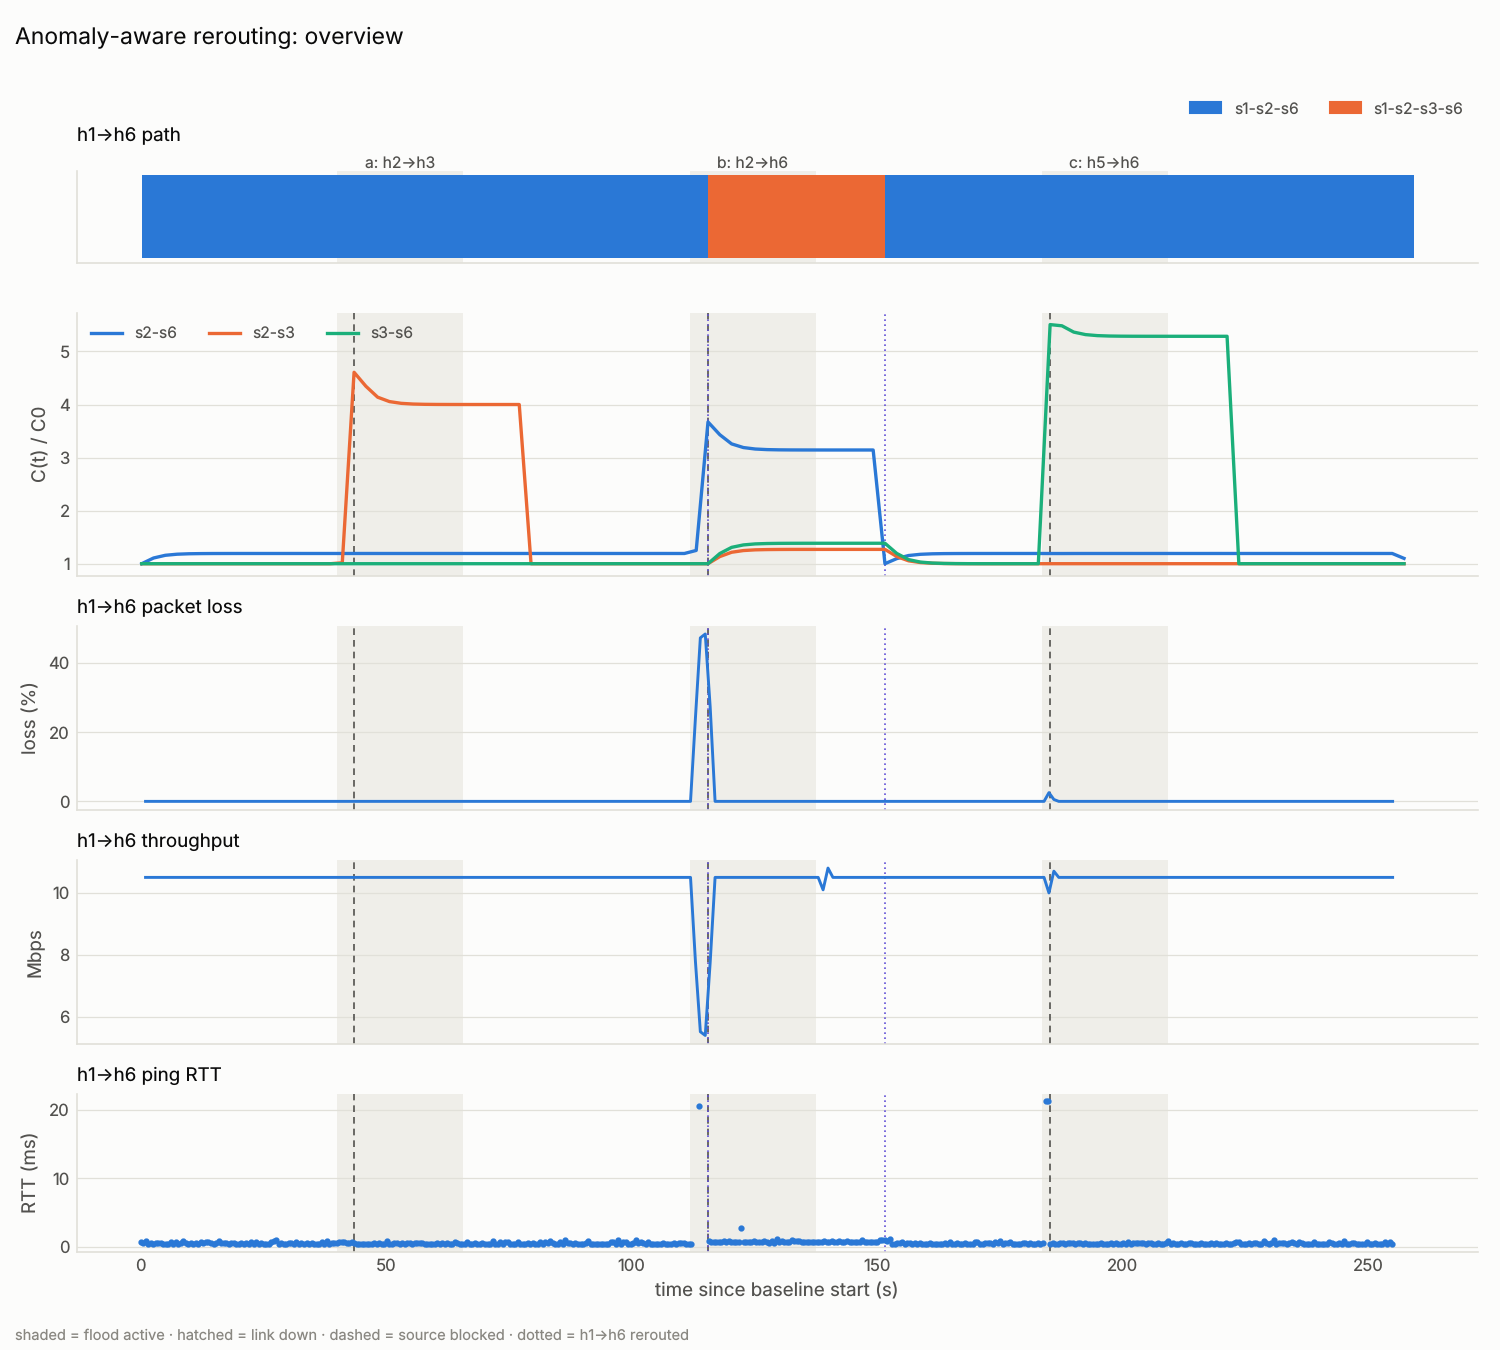
\includegraphics[width=0.95\textwidth]{figures/fig4_overview.png}
  \caption{Overview of R1: h1\ra h6 path, normalized cost of s2-s6, s2-s3 and s3-s6, packet loss, throughput
  and RTT on one time axis.}
  \label{fig:overview}
\end{figure}

The path band shows the single detour: h1\ra h6 used s1-s2-s3-s6 only from the block in case~b (115.6\,s) until
the anomaly hold on s2-s6 expired (151.6\,s). Loss and the throughput dip appear only in the 4\,s of case~b
before detection. RTT rose from about 0.5\,ms to about 20\,ms in that window, which is queueing delay in the full
40\,Mbps queue on s2-s6. Case~c caused one RTT spike of the same size at 184\,s, from the shared access link to
h6.

\subsection{Dynamic link cost vs.\ time}

\begin{figure}[H]
  \centering
  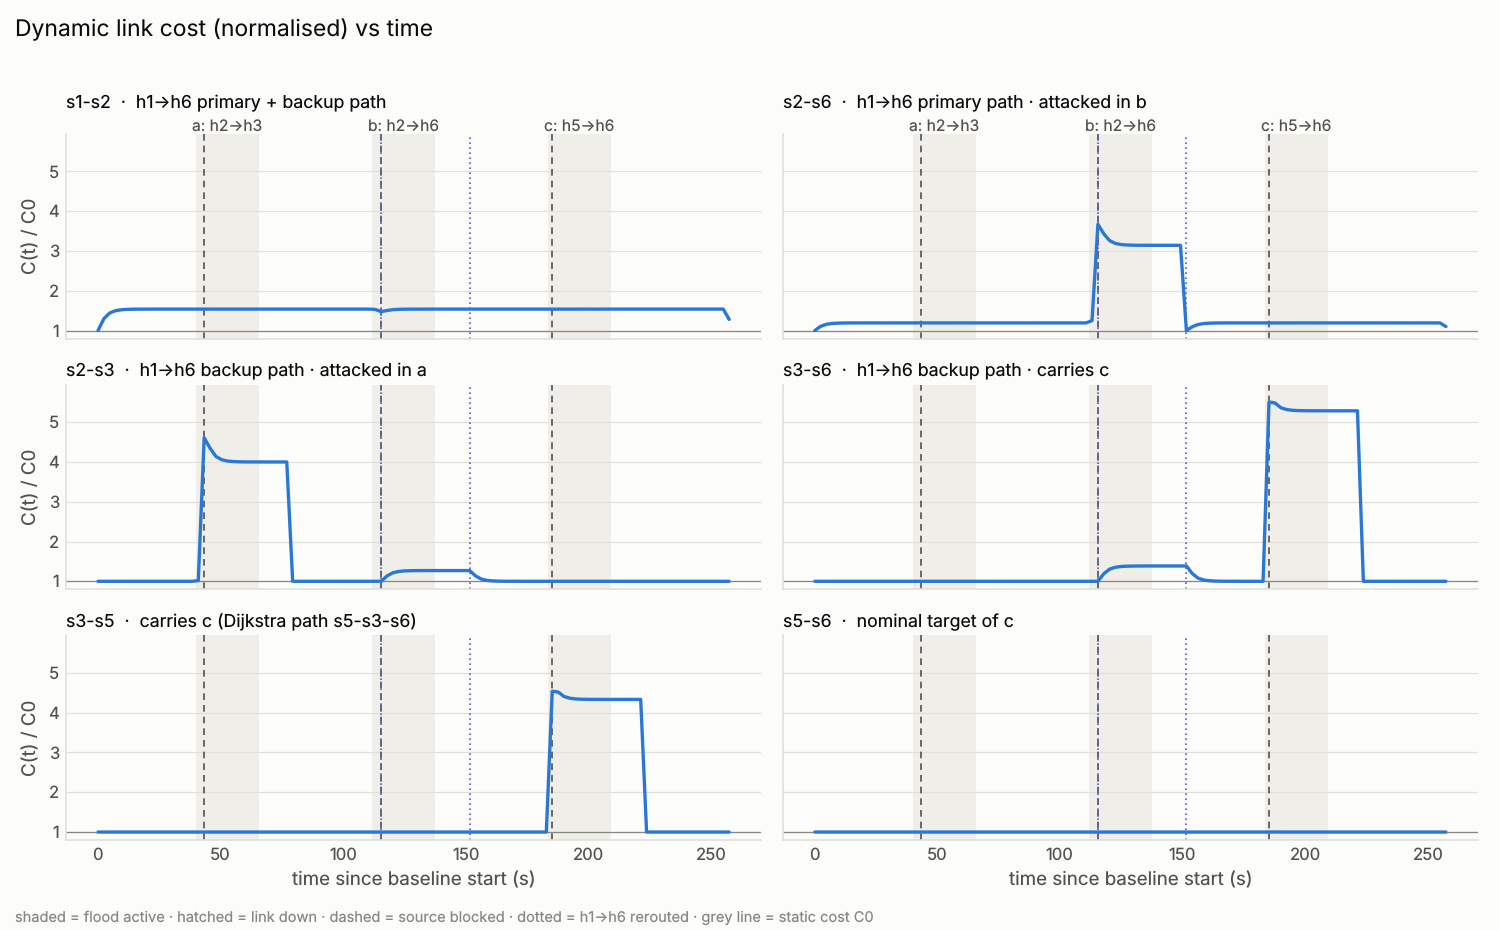
\includegraphics[width=0.95\textwidth]{figures/fig1_link_cost.png}
  \caption{Normalized dynamic cost $C(t)/C^0$ of six links over the R1 timeline.}
  \label{fig:cost}
\end{figure}

Every attacked link follows the same pattern (\figref{fig:cost}):
\begin{enumerate}
  \item \textbf{Spike at detection.} Both terms of Eq.~(\ref{eq:cost}) act at once: the link is still loaded and
        $A=1$. For example, s2-s6 reached $3.67\times C^0$.
  \item \textbf{Plateau while the attack lasts.} The block removes the load within one interval, so only $\beta$
        is left: $(C^0+30)/C^0$. That is 4.0 for s2-s3, 3.14 for s2-s6, 4.33 for s3-s5 and 5.29 for s3-s6. The
        same $\beta$ raises cheap links more in relative terms.
  \item \textbf{Return to baseline.} About 13--15\,s after the flood stops, which is the 10\,s hold plus up to two
        polling intervals.
\end{enumerate}

Links carrying the legitimate flow sit slightly above 1: s1-s2 at about 1.5 (10\,Mbps adds
$\alpha\times0.25=2.5$ to $C^0=5$) and s2-s6 at about 1.18. While h1\ra h6 was detoured in case~b, s2-s3 and
s3-s6 rose to 1.25--1.4 for the same reason. s5-s6 stayed at 1.0 throughout because no flow used it.

\subsection{Packet loss vs.\ time}

\begin{figure}[H]
  \centering
  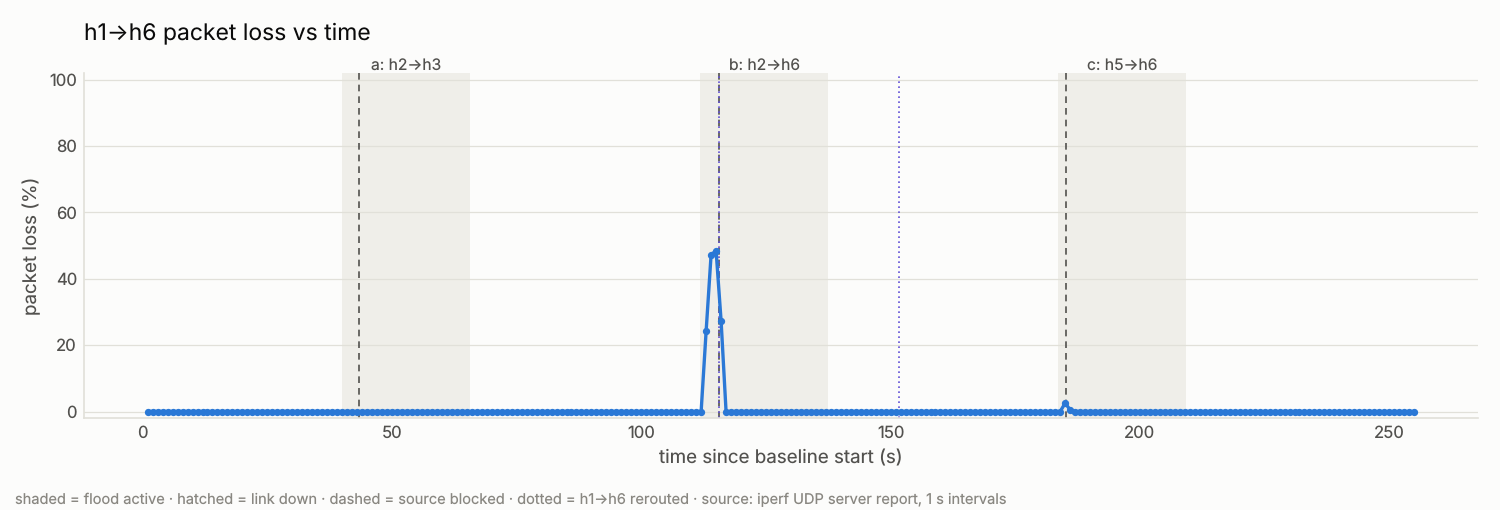
\includegraphics[width=0.95\textwidth]{figures/fig2_packet_loss.png}
  \caption{Packet loss of h1\ra h6 per second over the R1 timeline.}
  \label{fig:loss}
\end{figure}

Loss was 0\% except in two places (\figref{fig:loss}). Case~b: 24\%, 47\%, 48\% and 27\% in the four seconds
before detection, while flood and legitimate traffic shared s2-s6. Case~c: 2.5\% and 0.6\% in two seconds, from
the shared access link to h6. Case~a caused no loss because its flood shares no link with h1\ra h6. The reroute
itself lost no packets: the new path is installed egress first, before the ingress rule changes.

\subsection{Throughput vs.\ time}

\begin{figure}[H]
  \centering
  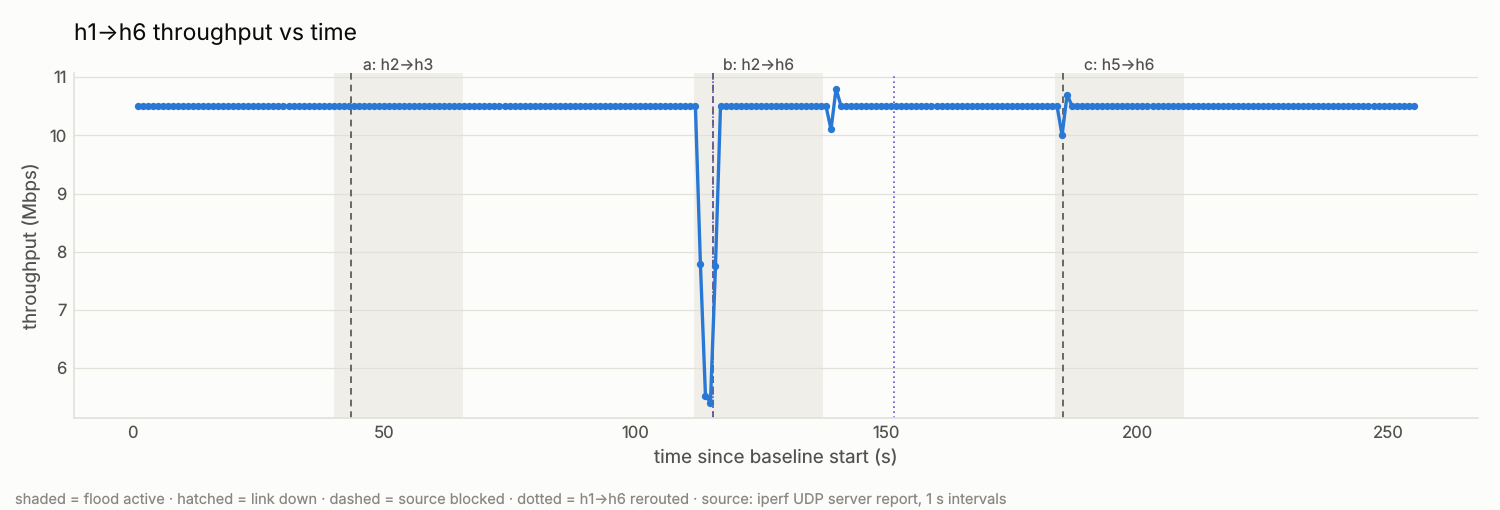
\includegraphics[width=0.95\textwidth]{figures/fig3_throughput.png}
  \caption{Throughput of h1\ra h6 per second over the R1 timeline.}
  \label{fig:tput}
\end{figure}

Throughput mirrors loss (\figref{fig:tput}): 10.5\,Mbps (the 10\,Mbps payload plus headers) except a dip to
5.4\,Mbps during the four lossy seconds of case~b and to 10.0\,Mbps in case~c. The 10.1/10.8\,Mbps pair at
139--140\,s has 0\% loss; packets moved between two 1\,s reporting intervals when the flood stopped. Moving back
to the original path at 151.6\,s caused no dip.

% =====================================================================
\section{Extended experiments}

Three controlled runs test the design choices: the anomaly weight $\beta$, case~c with traffic forced onto
s5--s6, and a link failure. Each uses one flood (or one failure) after a 30\,s baseline, with all other settings
as in Section~4. Section~\ref{sec:vm} then repeats the full a, b, c timeline on the Mininet VM with link delays.

\subsection{Sensitivity to $\beta$ (case b)}

$\beta$ decides whether h1\ra h6 leaves the attacked link. The backup path costs 3 more and the margin is 2, so
$\beta$ must exceed 5.

\begin{table}[H]
  \centering
  \small
  \caption{Case~b with different anomaly weights $\beta$.}
  \label{tab:beta}
  \begin{tabularx}{\textwidth}{l l >{\raggedright\arraybackslash}X >{\raggedright\arraybackslash}X l l}
    \toprule
    $\beta$ & Detection (s) & s2-s6 cost after the block ($\times C^0$) & h1\ra h6 during flood &
      Worst 1\,s loss (\%) & Loss after block (\%) \\
    \midrule
    0  & 1.5 & 1.20 & s1-s2-s6 (stayed) & 30.4 & 0 \\
    2  & 1.5 & 1.34 & s1-s2-s6 (stayed) & 30.1 & 0 \\
    30 (R1--R3) & 1.5--3.8 & 3.15--3.16 & s1-s2-s3-s6 (moved) & 34.4--56.6 & 0 \\
    \bottomrule
  \end{tabularx}
\end{table}

With $\beta=0$ the load term alone never moved the flow: the block cleared the load from s2-s6 within one
interval, before the cost could build up. With $\beta=2$ the anomaly flag raised the cost, but not past the
backup path. Only $\beta=30$ moved the flow, at the block itself.

Loss after the block was 0 in all three settings. In these experiments blocking at the attacker's switch is what
ends the loss; rerouting does not lower it further. The reroute moves the flow away from a link known to be under
attack until the attack has stopped. That guards against attack traffic the source-IP rule does not catch (for
example spoofed source addresses), at the price of a path that is 3\,ms longer. The worst-second loss depends
mainly on detection delay, not on $\beta$.

\subsection{Case c with traffic on s5--s6}
\label{sec:c-override}

To test the case as the assignment intends, \Czero{} of s5--s6 was lowered from 20 to 8
(environment variable \code{CEG\_COST\_OVERRIDE} set to \code{5-6:8}), so h5\ra h6 took s5-s6 directly. The controller detected h5 after 1.5\,s and
marked s5-s6, whose cost held at $4.76\times C^0$ during the flood. h1\ra h6 kept s1-s2-s6, which is correct
because the two paths share no switch-to-switch link.

h1\ra h6 still lost up to 35\% in the second before detection. Both flows end on h6's 40\,Mbps access link, so the
congestion is at the destination's last hop. No path choice avoids it; only the block ended it. This is a limit
of any rerouting scheme: it protects a flow only from congestion on links it can route around.

\subsection{Link failure on s2--s6}

The link-failure handling inherited from \code{resilient\_controller.py} still works inside the new cost model.
s2--s6 was taken down for 20\,s while h1\ra h6 ran at 10\,Mbps (\tabref{tab:linkfail}).

\begin{table}[H]
  \centering
  \small
  \caption{h1\ra h6 during a 20\,s failure of s2--s6.}
  \label{tab:linkfail}
  \begin{tabular}{lll}
    \toprule
    Event & Time & h1\ra h6 \\
    \midrule
    s2--s6 down & 30.1\,s & moved to s1-s2-s3-s6 7\,ms later \\
    While down (20\,s) & & 10.49\,Mbps, 0.06\% loss \\
    s2--s6 restored & 50.1\,s & back on s1-s2-s6 0.7\,s later \\
    \bottomrule
  \end{tabular}
\end{table}

The whole 80\,s run lost 11 of 71{,}515 packets, all in the second of the failure.

This experiment exposed a bug that the attack runs could not show, because no link went down in them. With one
link missing, the controller saw fewer than 11 links and fell back to its start-up ``topology not ready'' state,
in which it ignores packet-ins. About 16\,s into the outage h1's ARP entry for h6 expired, the new ARP request was
ignored, and traffic stopped until the link returned. The fix keeps the ready state once the first full discovery
has completed; the results above are from the fixed controller.

\subsection{Re-run on the Mininet VM with link delays}
\label{sec:vm}

The full a, b, c timeline of Section~4 was run once more on the Mininet 2.3.0 VM of Section~1, with the OVS
kernel datapath and the link delays of \tabref{tab:c0} emulated by \code{netem} (\code{results/vm-delay-abc}).
All other settings were as in R1--R3, except the 12-sample warm-up explained below.

\begin{table}[H]
  \centering
  \small
  \caption{The VM run with link delays compared with R1 (values given as R1\,/\,VM).}
  \label{tab:vm}
  \begin{tabularx}{\textwidth}{l l l >{\raggedright\arraybackslash}X >{\raggedright\arraybackslash}X
      >{\raggedright\arraybackslash}X}
    \toprule
    Case & Detection (s) & h1\ra h6 rerouted & Worst 1\,s loss (\%) & Lowest 1\,s Mbps &
      Max RTT before detection (ms) \\
    \midrule
    a: h2\ra h3 & 3.4 / 2.2 & no / no   & 0 / 0       & 10.5 / 10.4 & 0.7 / 114 \\
    b: h2\ra h6 & 3.8 / 1.6 & yes / yes & 48.4 / 11.2 & 5.41 / 9.84 & 20.5 / 383 \\
    c: h5\ra h6 & 1.7 / 3.8 & no / no   & 2.5 / 10.4  & 10.0 / 8.95 & 21.3 / 408 \\
    \bottomrule
  \end{tabularx}
\end{table}

The control behaviour was the same as in R1--R3. The controller blocked the same hosts (h2, h2, h5) and marked
the same links (s2-s3, s2-s6, and s3-s5 with s3-s6). It rerouted h1\ra h6 only in case~b, at the block itself
(path cost 54.96 for staying versus 30.2 for moving), and moved it back to s1-s2-s6 40.8\,s after the flood
began, 0.9--2.1\,s later than in R1--R3 (38.6--39.9\,s). These were the only two h1\ra h6 reroutes. While s2-s6
was marked its cost held at $3.14\times C^0$, as in R1. Detection in case~c took 3.85\,s, slightly longer than in
any container run (at most 3.76\,s): the flood began just before a statistics snapshot, so the first sample saw
only 37\,pkt/s and the next one (3{,}092\,pkt/s) triggered the block. No attack packet reached the victim later
than 1\,s after a block. Packets already queued in \code{netem} were still delivered up to 0.5\,s after it
(487--1{,}188 per case, against 26--87 in R1).

With real delays, the median RTT of h1\ra h6 was 99.8\,ms before the first flood, against the 98\,ms that the
delays of s1-s2-s6 give ($2\times(15+5+14+15)$). On the detour s1-s2-s3-s6 the median was 109.0\,ms. The longer
path accounts for 6\,ms of the increase; the rest came while the flood was still running, since the median was
107\,ms after the flood ended. After the return the median was 100.0\,ms again.

Software emulation weakened the flood, so the loss figures cannot be compared with R1--R3. Before each block the
attacker's interface sent only 3{,}000--3{,}900\,pkt/s (R1: about 4{,}800, the 40\,Mbps limit), and about
2{,}500\,pkt/s (21\,Mbps) of flood reached h6 in cases b and c, about 70\% of R1's rate. Each delayed link also
has a \code{netem} queue, which Mininet leaves at its default of 1{,}000 packets, or 200--300\,ms at 40\,Mbps.
So the flood filled a deep queue instead of overflowing a short one. Before detection, h1\ra h6 saw RTTs of up to
383\,ms (b) and 408\,ms (c), against about 20\,ms in the container, but in case~b it lost less (11.2\% against
34.4--56.6\% in R1--R3). Case~b was also detected quickly in the VM; R3, the container run with a similar
detection delay (1.5\,s), lost 34.4\%. In case~c the longer detection and the deep queue gave a worse second
(10.4\%) than any container run (2.5--6.1\%). Some RTT spikes are emulation stalls rather than queueing, for
example 328\,ms at 65.6\,s, when no flood shared h1's path.

\paragraph{Warm-up on a delayed network.} The first VM run used the default 5-sample warm-up and is not valid
(\code{results/vm-delay-abc-warmup5}, kept as evidence). The delays slowed the two \code{pingAll} rounds that
run before the traffic, so h1's iperf started 14.2\,s after the topology was ready, against 1.2\,s in the
container. h1's five warm-up samples had ended 2.9\,s before that, so its iperf flow (about 890\,pkt/s) was
judged as new traffic. A partial sample of 377\,pkt/s was learned, the next sample of 920\,pkt/s exceeded the
resulting 804\,pkt/s threshold, and h1 was blocked 4.4\,s after its iperf started. h1\ra h6 carried nothing for
the rest of that run, and s1-s2 and s2-s6 stayed marked, which also changed the paths of the later floods. The
runner now sets \code{CEG\_WARMUP=12} when link delays are emulated, \code{CEG\_WARMUP} is not set and the runner
starts the controller itself. For the run in \tabref{tab:vm} the value was set by hand; h1's warm-up then ended
28\,s after the topology was ready, 14\,s after its iperf started. A later case-b run without setting \code{CEG\_WARMUP} confirmed the default
(\code{results/vm-autowarmup-b}): the controller ran with 12 warm-up samples, h1 was not blocked, h2 was blocked
after 3.2\,s and h1\ra h6 was rerouted and moved back as before.

% =====================================================================
\section{Discussion and limitations}

The weakest point is the 1.5--3.8\,s detection delay, because every lost packet in the experiments fell inside it.
Everything after detection (block, cost change, reroute, recovery) took effect within one 2\,s interval.

\paragraph{Detection delay vs.\ false alarms.} The delay is one or two polling intervals. A shorter interval or a
per-packet sampling mechanism would cut it, at the cost of more control traffic and noisier rate estimates.
Requiring two consecutive anomalous samples (\code{CEG\_CONSEC=2}) would make false alarms rarer but add 2\,s of
loss to every real attack. In R1--R3, h1's iperf flow (about 890\,pkt/s) never triggered an alarm: it started
during the warm-up, so h1's baseline was learned from it. A legitimate flow that starts later at that rate is
flagged, which is the price of a baseline-relative detector. The first VM run showed this false alarm: the link
delays slowed the start-up pings, h1's flow began after its 5-sample warm-up, and h1 was blocked for the rest of
the run (Section~\ref{sec:vm}). A longer warm-up only covers flows that start soon after the host appears.

\paragraph{What the cost model captures.} Eq.~(\ref{eq:cost}) mixes a fast signal (load, gone one interval after
the block) with a slow one ($A$, held for the attack's duration plus 10\,s). The slow term is what makes rerouting
stable: without it the flow would move back to the attacked link as soon as the block cleared the load
(Section~7.1). The hysteresis margin and the ``own load'' correction kept every flow from oscillating; each case~b,
including the VM run, produced exactly two h1\ra h6 reroutes, away and back.

\paragraph{Path choice costs latency.} The detour s1-s2-s3-s6 costs 22 instead of 19, about 3\,ms more each way
with the topology's delays. On the VM, with real delays, the median RTT rose from 99.8\,ms to 109.0\,ms on the
detour (Section~\ref{sec:vm}). The controller accepts that only while $A=1$ and returns as soon as the hold ends.

\paragraph{Limitations.}
\begin{itemize}
  \item Blocking is per source IP. A flood with spoofed or randomised source addresses would not be stopped by
        it; then the anomaly-aware reroute is the remaining protection, and per-destination rate limiting would
        be needed.
  \item The block also stops the attacker's legitimate traffic (h2's background ping) until it is lifted 10\,s
        after the flood ends.
  \item The 500\,pkt/s floor, the hold time and $\beta$ are tuned for this topology and these traffic rates, not
        derived.
  \item Congestion on the destination's access link (case~c and Section~\ref{sec:c-override}) cannot be routed
        around.
  \item A partial first sample just under the threshold can be learned into the baseline (R1 case~b). Bounding
        how far one sample may move the baseline would close that gap.
  \item R1--R3 ran on a userspace OVS datapath without delay emulation. The VM run added the kernel datapath and
        real link delays and reproduced the control behaviour, but under software emulation: the flood reached
        the victim at only about 70\% of the container rate, and the deep \code{netem} queues changed how loss
        and delay show up before detection. Neither environment gives the loss and RTT figures of real
        hardware.
\end{itemize}

% =====================================================================
\section{Conclusion}

The controller met every requirement of the assignment in all three repeated runs. It detected each ICMP flood
within 1.5--3.8\,s and blocked the source, after which no attack packet reached the victim. It raised the dynamic
cost of the attacked links, rerouted h1\ra h6 only when the attack shared its path (case~b), and restored the
original path 13.6--14.9\,s after the flood ended. Outside the few seconds before each detection, h1\ra h6 kept
10.5\,Mbps with 0\% loss. A re-run on the Mininet 2.3.0 VM with the kernel datapath and real link delays gave the
same blocks, marked links and reroutes, with detection in 1.6--3.8\,s.

The experiments also showed what each part contributes. Blocking ends the loss. The anomaly term $\beta\cdot A$
keeps traffic off an attacked link after the block has removed its load. The hysteresis and own-load correction
keep routing stable. Faster detection is the most useful next step, since the time before detection is where all
observed loss occurred.

% =====================================================================
\appendix
\section{Code and reproduction}

\begin{table}[H]
  \centering
  \small
  \begin{tabularx}{\textwidth}{l >{\raggedright\arraybackslash}X}
    \toprule
    File & Content \\
    \midrule
    \code{code/controller/integrated\_controller.py} & Ryu application: topology, ARP, routing, monitoring, blocking,
      dynamic cost, rerouting, logs \\
    \code{code/controller/sdn\_logic.py} & Parameters, static costs $C^0$, Eq.~(\ref{eq:cost}), Dijkstra, anomaly
      detector (no Ryu dependency) \\
    \code{support/tests/test\_sdn\_logic.py} & 18 unit tests of costs, paths and detection \\
    \code{code/experiments/run\_experiment.py} & Builds the topology, runs the traffic timeline, collects all logs \\
    \code{support/analysis/plot\_results.py} & Figures and summary table from a run directory \\
    \code{code/miniedit/my\_topology.mn} & The topology built in the MiniEdit GUI (Figures~\ref{fig:miniedit-canvas}
      and~\ref{fig:miniedit-run}); \code{my\_topology\_export.py} is its Level~2 script export \\
    \code{support/miniedit/ceg\_mesh\_topo.mn} & The same topology for MiniEdit, generated by \code{make\_mn.py} \\
    \code{presentation/assets/video/miniedit\_build.mp4} & A 12$\times$ time-lapse of the MiniEdit build \\
    \code{support/environment/qemu\_mininet\_vm.sh} & Boots the official Mininet 2.3.0 VM under QEMU \\
    \code{results/} & Raw data of every run in this report (R1 = \code{validation-abc}, R2 = \code{run1-abc},
      R3 = \code{run2-abc}, \code{exp-*}, the VM run \code{vm-delay-abc}, its check \code{vm-autowarmup-b}, and \code{miniedit-vm} for the MiniEdit
      build). \code{vm-delay-abc-warmup5} is the invalid first VM run; it was renamed after the run, so its
      \code{meta.json} still names \code{vm-delay-abc} \\
    \bottomrule
  \end{tabularx}
\end{table}

To reproduce, from the project root:
\begin{lstlisting}[language=bash]
bash support/environment/setup_ubuntu.sh
export RYU_MANAGER=~/ryu-venv/bin/ryu-manager PLOT_PYTHON=~/ryu-venv/bin/python
sudo -E python3 code/experiments/run_experiment.py   # CEG_WARMUP=12 by default when link delays are on
sudo -E env CEG_BETA=2 python3 code/experiments/run_experiment.py --scenarios b --baseline 30
sudo -E env CEG_COST_OVERRIDE=5-6:8 python3 code/experiments/run_experiment.py --scenarios c --baseline 30
sudo -E python3 code/experiments/run_experiment.py --scenarios "" --baseline 30 \
     --fail-link s2-s6 --fail-for 20 --recover 30
\end{lstlisting}

When link delays are emulated, as on the Mininet VM, and \code{CEG\_WARMUP} is not set, the runner starts the
controller with \code{CEG\_WARMUP=12} (Section~\ref{sec:vm}); \code{sudo -E env CEG\_WARMUP=N} overrides it. With
\code{-{}-controller external} the runner cannot pass the value on, so start that controller with
\code{CEG\_WARMUP=12} yourself. \code{bash support/environment/qemu\_mininet\_vm.sh} boots the VM; copy the project into it
over SSH (port 2222) and run the same commands there.

\end{document}
